In this section the final system is tested with varying input signal, according to evaluate at what level the application fulfil the practical purpose of the system. Cf. chapter \ref{ch3} the purpose of the system is to create a spectrogram from which the significant frequencies over time are to be recognized by the peak detection algorithm to match the frequencies known to be in the input signal - according to the tone or chord played.\\
In each test the same noise is added to the signal, with a maximum signal to noise ration at ---- \trine{insæt max SNR}. The noise consist of hands clapping in the background, to simulate a realistic situation. Note that all other natural noise is hence is minimized. Variation of the noise will not be considered in this system validation but will be further investigated in chapter \ref{ch11}.         
\paragraph{Test 1} Scale with clapping hands
\begin{figure}[H]
\centering
\begin{subfigure}{0.49\textwidth}
\centering
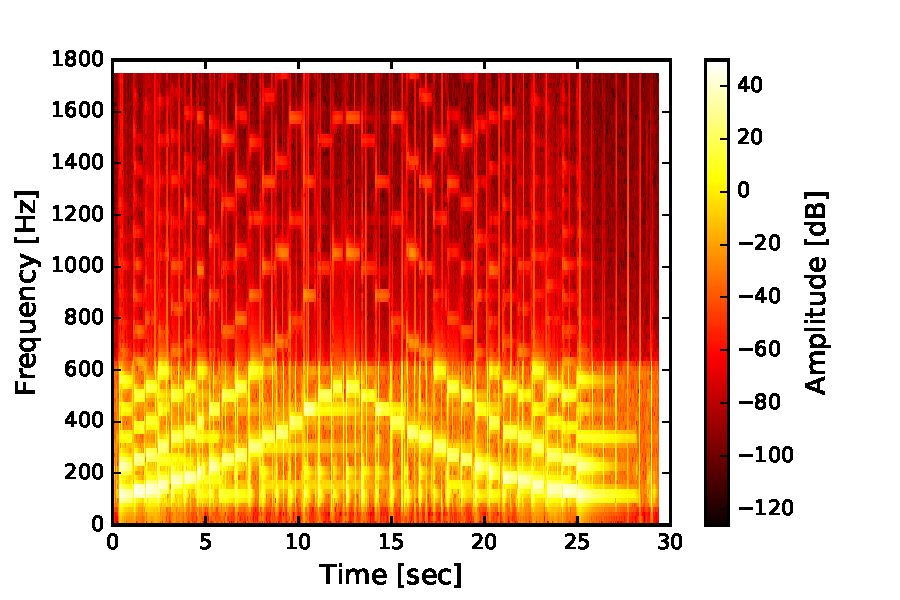
\includegraphics[width=\textwidth]{figures/validation/systemtest/final_spec.pdf}
\caption{Spectrogram}
\label{fig:final_spec1}
\end{subfigure}
\begin{subfigure}{0.49\textwidth}
\centering
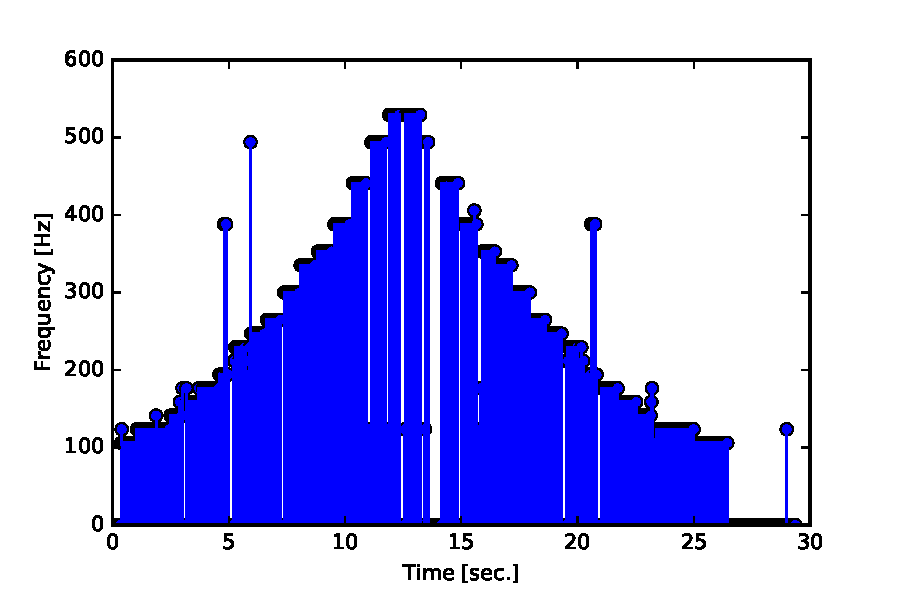
\includegraphics[width=\textwidth]{figures/validation/systemtest/final_peak.pdf}
\caption{Significant frequencies}
\label{fig:final_peak1}
\end{subfigure}
\caption{Scale with clapping hands}
\label{fig:final_1}
\end{figure} 

Figure \ref{fig:final_1} account for the system output of test 1. From the results it is clear that the significant frequencies follows an octatonic scale. Though single incongruous frequencies appears, caused by a low signal to noise ratio within the passband at a certain time.
It is clear that the lowest frequencies lay closer as expected, hence it is a bit harder to identify the actual frequency. \\ 
From the result it is concluded that the scale is recognisable. 

\paragraph{Test 2} Melody "Lille Peter edderkop" by single tones with clapping hands.  
\begin{figure}[H]
\centering
\begin{subfigure}{0.49\textwidth}
\centering
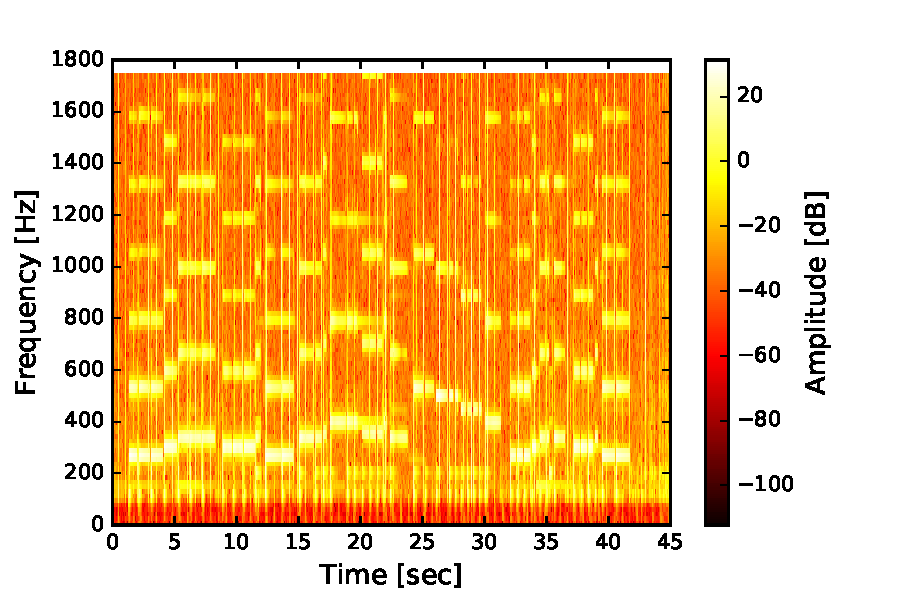
\includegraphics[width=\textwidth]{figures/validation/systemtest/final_spec3.pdf}
\caption{Spectrogram}
\label{fig:final_spec2}
\end{subfigure}
\begin{subfigure}{0.49\textwidth}
\centering
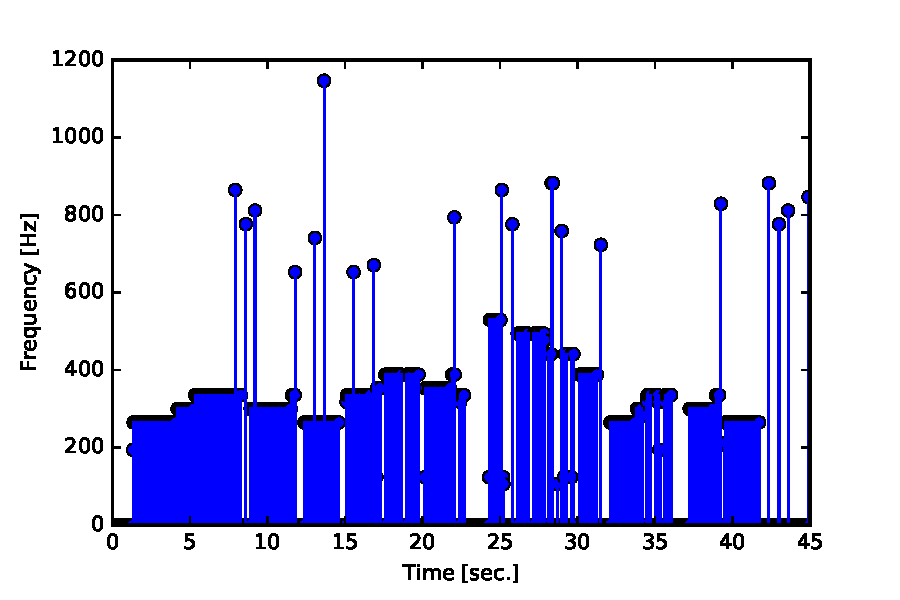
\includegraphics[width=\textwidth]{figures/validation/systemtest/final_peak3.pdf}
\caption{Significant frequencies}
\label{fig:final_peak3}
\end{subfigure}
\caption{Melody "Lille Peter edderkop" by single tones with clapping hands.}
\label{fig:final_3}
\end{figure}  

Figure \ref{fig:final_3} accounts for the output of test 2. It is seen compared to the result of the scale that the significant frequencies are not as clear caused by several incongruous detected frequencies. Though by ignoring the single peaks in  \ref{fig:final_peak3} it is possible to sense the pattern of the frequencies. The first three different frequencies detected is approximately 258 Hz, 301 Hz and 322 Hz 
this corresponds within a range of $\pm 10$ Hz to the first line of the melody being C C C D E E E - which also corresponds with the time axis. \\
By this one can conclude that the melody is recognisable on behalf of the result, but a selective algorithm is required to determine the right tones.                  

\paragraph{Test 3} Low E chord with clapping hands
\begin{figure}[H]
\centering
\begin{subfigure}{0.49\textwidth}
\centering
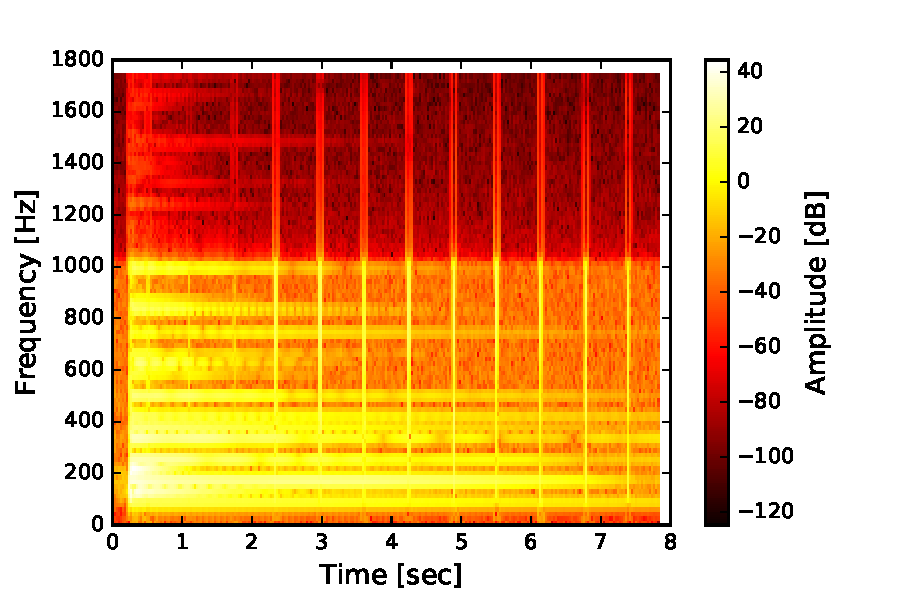
\includegraphics[width=\textwidth]{figures/validation/systemtest/final_spec2.pdf}
\caption{Spectrogram}
\label{fig:final_spec2}
\end{subfigure}
\begin{subfigure}{0.49\textwidth}
\centering
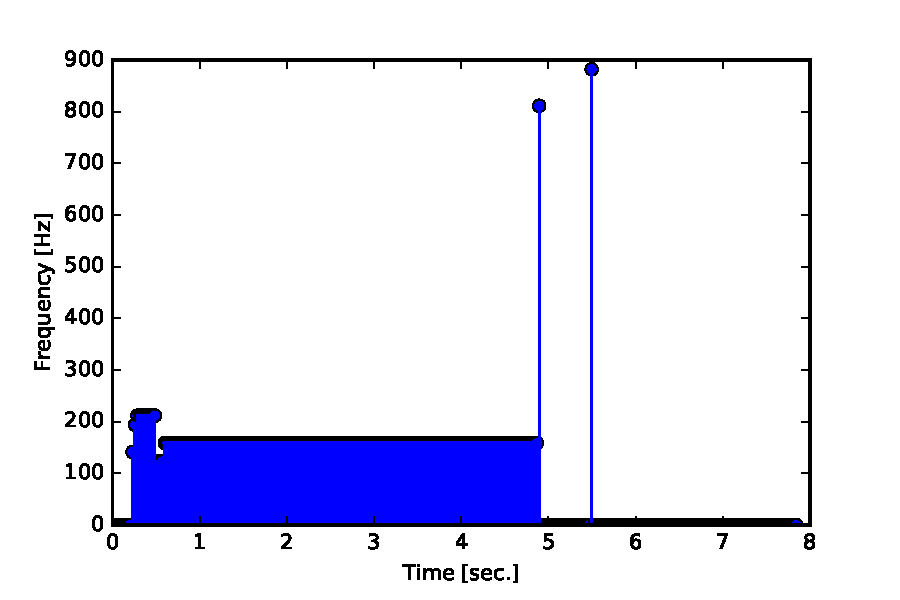
\includegraphics[width=\textwidth]{figures/validation/systemtest/final_peak2.pdf}
\caption{Significant frequencies}
\label{fig:final_peak2}
\end{subfigure}
\caption{Low E chord with clapping hands}
\label{fig:final_2}
\end{figure}  

Figure \ref{fig:final_2} accounts for the output of test 3. By the detected frequencies it is most likely to indicate that it is a single low E tone played, cf. figure \ref{fig:inte_peak}, rather than the low E chord played. As explained in chapter \ref{ch2} an chord is an harmonic of at least three tones, in this case E, B, G\# and over tones. Hence the peak detection algorithm is not sufficient to detect chords. Neither the spectrogram provide readable information, because the tones above the significant E tone are difficult to identify. Further it would require intelligent guessing in order to connect the correct frequencies found to be the most significant. \trine{some one?} 

\subsection{Evaluation}
From the test results of the final application it is seen that the system is capable of computing a spectrogram on behalf of a given input signal. Noise outside a given passband are successfully removed in order to isolate the frequencies expected within the musical range\trine{formulering?}. From the chosen trade off between accuracy in time and frequency   it is possible to detect the significant frequency corresponding to a given single tone within an approximate range of $\pm 10$ Hz. This is sufficient under the assumption that only the standard tones are used. The exactness in time are not fully obtained but visually it appears sufficient.\\        
Test 1 and test 2 indicates further that when the input signal gets more complex - according to speed and shift between tones - it is more difficult to detect the right tones. \\
By test 3 it is concluded that the application is not capable of determine a specific chord.\\   
\\
As an conclusion the application is found to fulfil the primary purpose when the input signal is limited to consist of single standard tones recorded under controlled circumstances.\\
The resistance towards varying noise will be investigated in the following chapter.           